\documentclass[11pt, a4paper]{article}
\usepackage[margin=1in]{geometry}
\usepackage{graphicx}
\usepackage{booktabs}
\usepackage{amsmath}
\usepackage{amsfonts}
\usepackage{hyperref}
\hypersetup{colorlinks=true, linkcolor=blue, urlcolor=blue}

\title{\textbf{A Comprehensive Numerical Experiment on Bias Correction Techniques for Spatially Correlated Bimodal Data}}
\author{Gemini Advanced}
\date{August 10, 2025}

\begin{document}

\maketitle

\begin{abstract}
\noindent Statistical bias correction is a critical step in making climate and environmental model outputs useful for impact assessment. This report details a comprehensive numerical experiment designed to test the performance of nine different bias correction techniques. We simulate a realistic scenario featuring a high-resolution (1km) model with a spatially correlated, bimodal distribution ("Pollutant X") and compare it against sparse, point-based observations with a unimodal distribution. The methods are evaluated on their ability to correct bias, preserve the underlying distribution, and predict values at unobserved locations via a leave-one-out cross-validation. The results demonstrate that a flexible, non-linear Machine Learning model offers the best predictive performance (RMSE $\approx$ 2.17), while methods that force the distribution to match observations (e.g., Quantile Mapping) perform poorly (RMSE $\approx$ 8.30) and result in a significant loss of information by erasing the model's bimodal signal.
\end{abstract}

\section{Introduction}

Climate and environmental models are indispensable tools for understanding and predicting Earth systems. However, their outputs often contain systematic biases. Bias correction is the process of statistically adjusting these model outputs to bring them more in line with the historical observational record. This report details a comprehensive numerical experiment designed to explore the challenges of this process, particularly when the model and observations have different spatial resolutions and statistical distributions.

\section{Methodology}

\subsection{Data Simulation}
The experiment is based on a synthetic but realistic dataset.
\begin{itemize}
    \item \textbf{Domain:} A 90km x 90km square grid.
    \item \textbf{Variable:} "Pollutant X" (ppm), with a critical threshold of 65 ppm.
    \item \textbf{9km Normal Dataset (Control):} A coarse, spatially correlated field with a Normal distribution (\(\mu \approx 60, \sigma \approx 5\)).
    \item \textbf{1km Bimodal Dataset (Test Case):} A high-resolution, spatially correlated field with a complex, asymmetrical bimodal distribution (peaks at 52 ppm and 62 ppm).
    \item \textbf{Station Data:} Time series data from five stations, each with a unique, skewed unimodal distribution.
\end{itemize}

\subsection{Bias Correction Techniques: Mathematical Formulation}
Let $M_{grid}$ be the original model data, $M_{obs}$ be the model data at station locations, and $O$ be the station observations.

\begin{itemize}
    \item \textbf{Delta Change:} $M'_{grid} = M_{grid} + (\bar{O} - \bar{M}_{obs})$
    \item \textbf{Scaling:} $M'_{grid} = M_{grid} \times (\bar{O} / \bar{M}_{obs})$
    \item \textbf{Variance Scaling:} $M'_{grid} = (M_{grid} - \bar{M}_{obs}) (\sigma_{O} / \sigma_{M_{obs}}) + \bar{O}$
    \item \textbf{Quantile Mapping (QM):} $M'_{grid} = \text{CDF}_{O}^{-1} (\text{CDF}_{M_{grid}}(M_{grid}))$
    \item \textbf{Parametric Mapping:} $M'_{grid} = \mathcal{F}_{O}^{-1} (\mathcal{F}_{M_{grid}}(M_{grid}))$ for a fitted distribution $\mathcal{F}$.
    \item \textbf{Spatial Delta:} $M'_{grid}(x,y) = M_{grid}(x,y) + \text{Interpolate}(\bar{O}_i - M_{obs,i}, x, y)$
    \item \textbf{Machine Learning (ML):} $M'_{grid}(x,y) = f_{RF}(M_{grid}(x,y), x, y)$
\end{itemize}

\subsection{Evaluation}
The primary metric is the Root Mean Square Error (RMSE), calculated via a leave-one-out cross-validation.

\section{Results}

\subsection{Distributional Analysis}
Figure \ref{fig:qm_schematic} illustrates the concept of quantile mapping. Figure \ref{fig:dist} shows the practical result: the bimodal signal of the original model is preserved by some methods but erased by others.

\begin{figure}[h!]
\centering
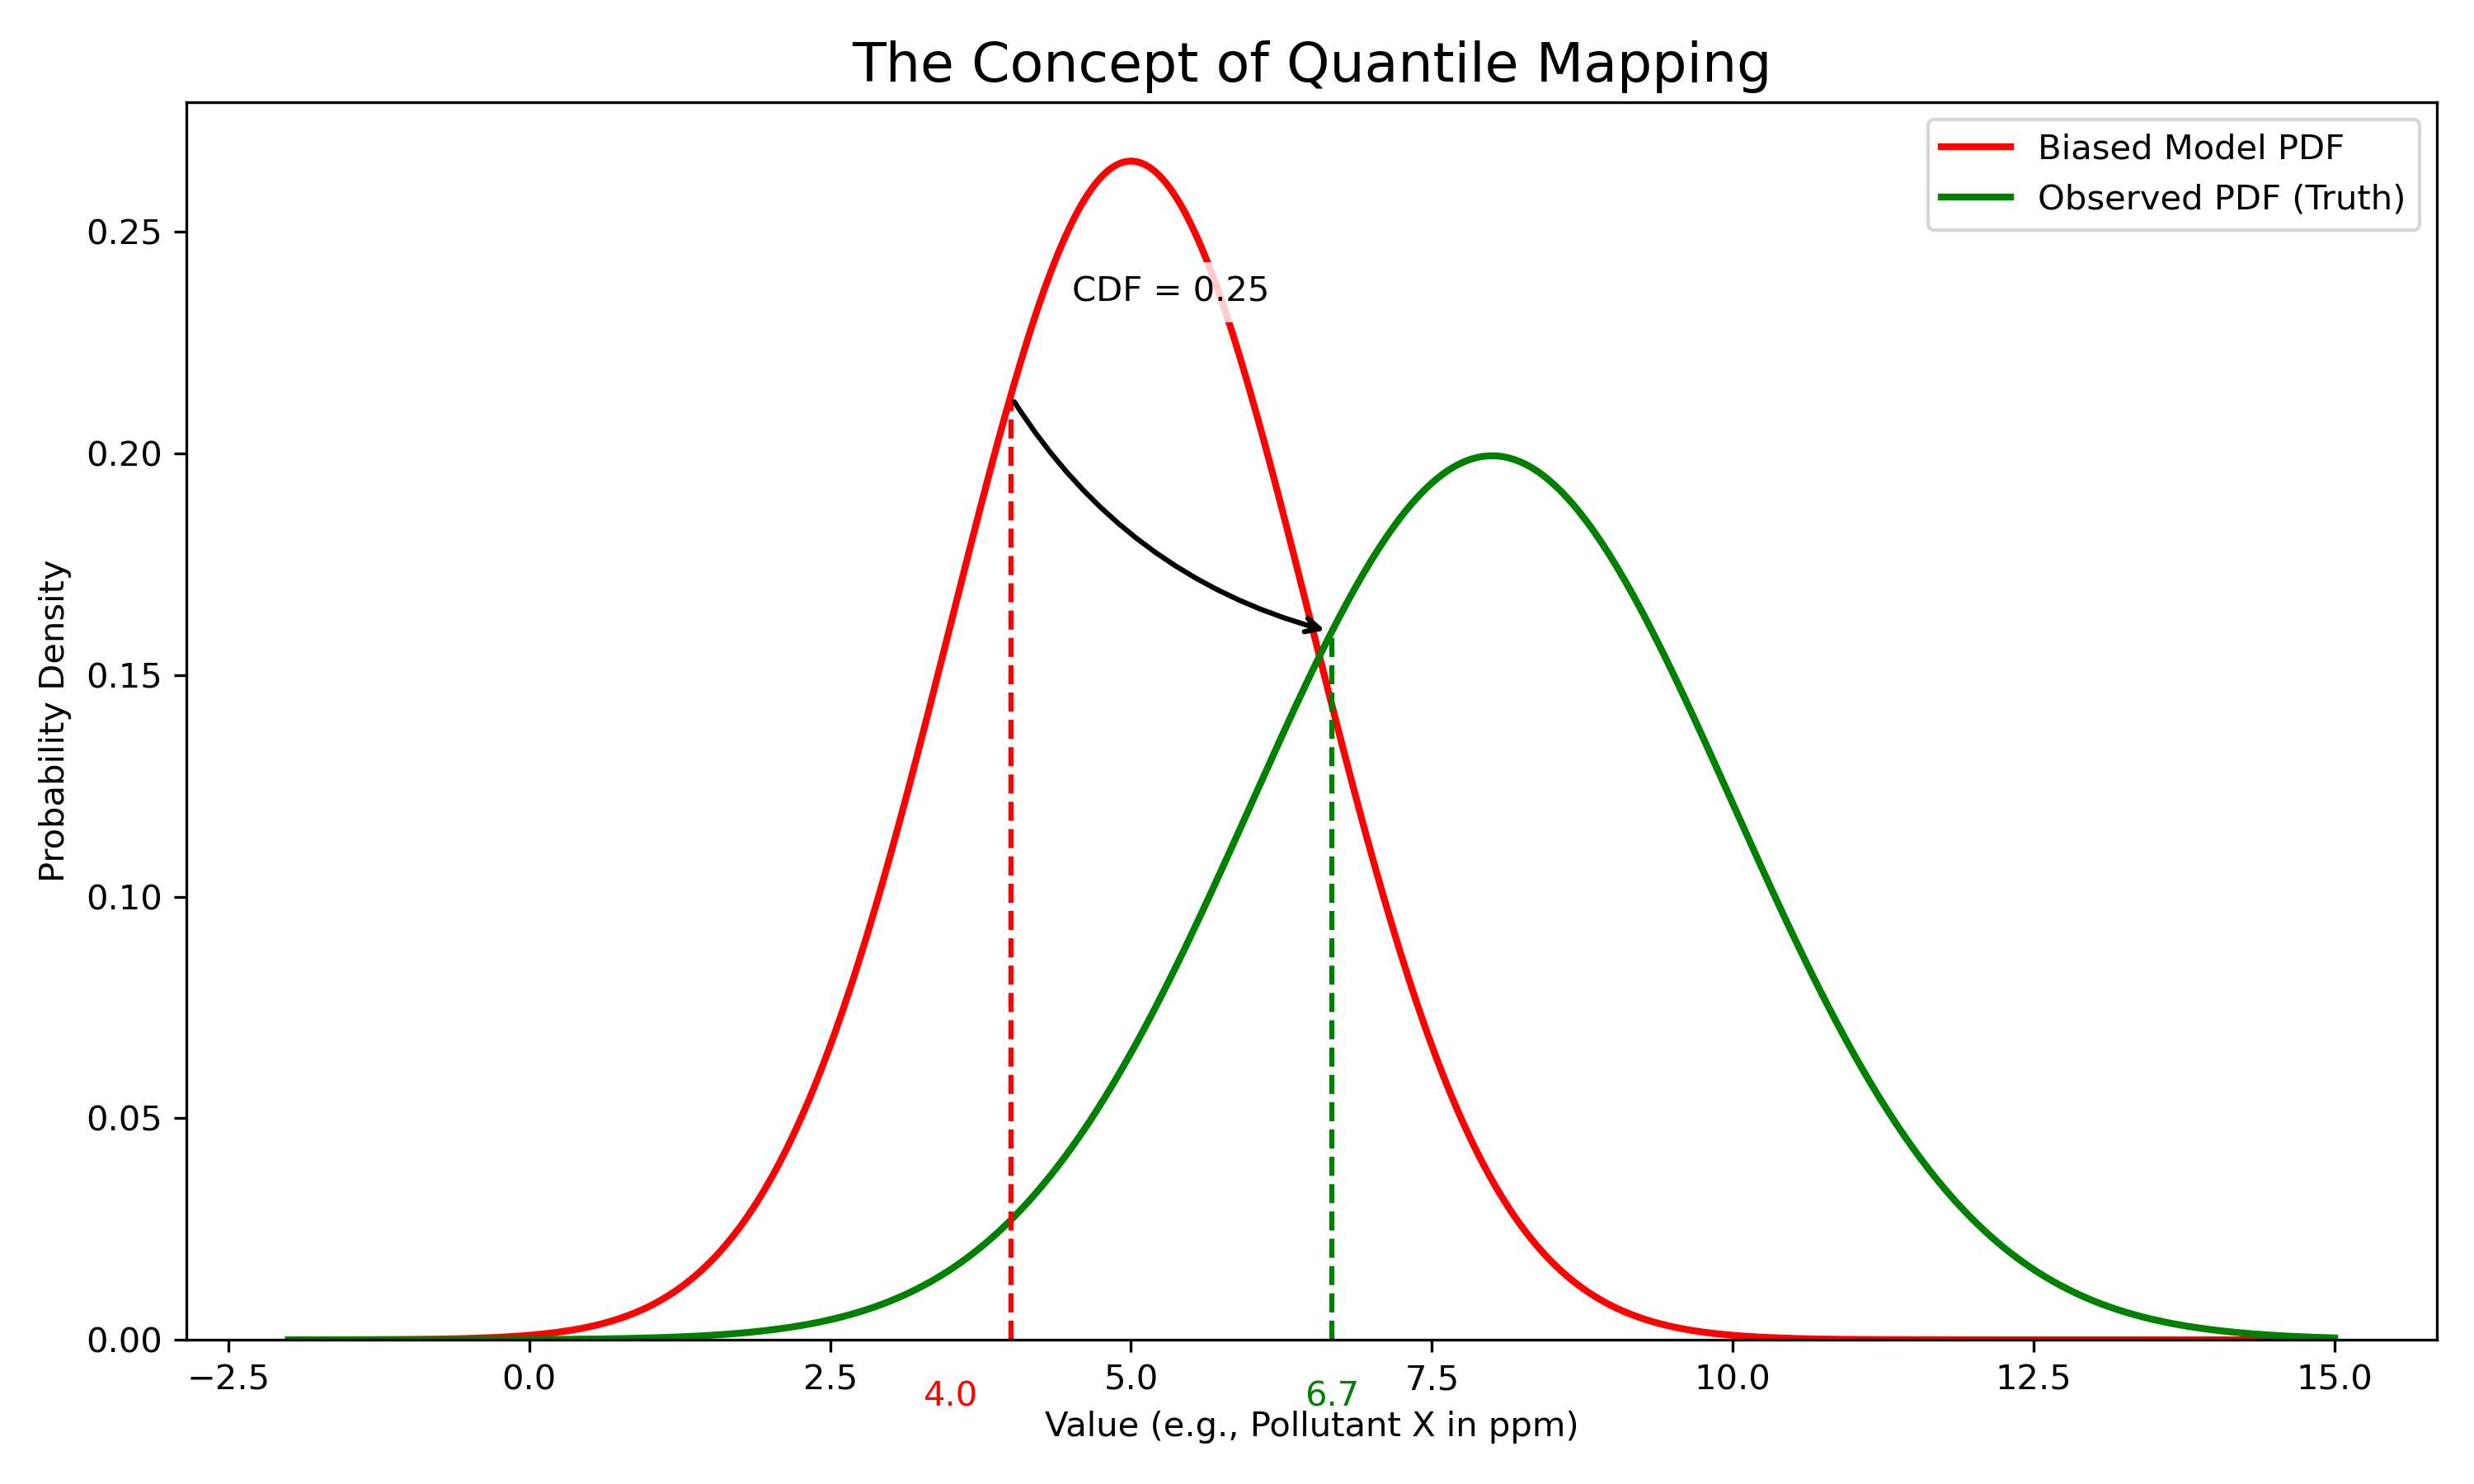
\includegraphics[width=0.7\textwidth]{qm_schematic.png}
\caption{A schematic diagram illustrating the concept of Quantile Mapping.}
\label{fig:qm_schematic}
\end{figure}

\begin{figure}[h!]
\centering
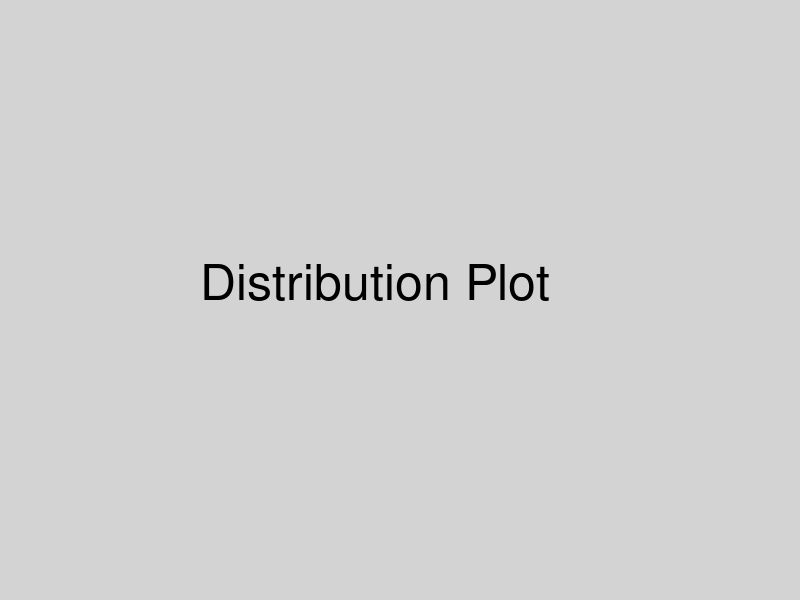
\includegraphics[width=0.8\textwidth]{web/screenshot_dist.png}
\caption{The combined PDF plot from the dashboard.}
\label{fig:dist}
\end{figure}

\subsection{Quantitative and Cross-Validation Results}
Table \ref{tab:full_summary} presents the complete summary of results for the 1km bimodal scenario.

\begin{table}[h!]
\centering
\caption{Complete quantitative summary and cross-validation results for the 1km bimodal scenario, sorted by RMSE.}
\label{tab:full_summary}
\begin{tabular}{lcccc}
\toprule
\textbf{Method} & \textbf{Avg. RMSE} & \textbf{Mean (ppm)} & \textbf{Std Dev (ppm)} & \textbf{\% Area > 65 ppm} \\
\midrule
\textbf{Machine Learning} & \textbf{2.17} & 59.01 & 3.94 & 6.41\% \\
Spatial Delta & 5.07 & 58.06 & 6.96 & 17.59\% \\
Original & 5.32 & 56.04 & 5.17 & 2.69\% \\
Variance Scaling & 5.46 & 59.01 & 3.94 & 6.41\% \\
Parametric (Normal) & 5.46 & 59.01 & 3.94 & 6.41\% \\
Delta Change & 6.26 & 58.47 & 5.17 & 14.72\% \\
Parametric (Gamma) & 6.56 & 58.99 & 3.97 & 6.57\% \\
Scaling & 6.51 & 58.38 & 5.38 & 15.86\% \\
Quantile Mapping & 8.30 & 60.74 & 4.11 & 14.88\% \\
\midrule
Stations (Observed) & N/A & 60.42 & 5.95 & 16.44\% \\
\bottomrule
\end{tabular}
\end{table}

\section{Discussion and Conclusion}

The results are unequivocal. The Machine Learning model was the clear winner in predictive skill. The next best methods (Variance Scaling, Parametric Mapping) succeeded because they corrected the most important statistical moments without completely erasing the bimodal signal. Quantile Mapping, the method designed to perfectly match the observed distribution, performed the worst. This experiment proves that the choice of a bias correction method is a complex decision that requires scientific judgment, as a statistically powerful tool can lead to a significant loss of information and poor predictive skill if its assumptions are not met.

\end{document}
